\documentclass[10pt,twocolumn,letterpaper]{article}

\usepackage{cvpr}
\usepackage{times}
\usepackage{epsfig}
\usepackage{graphicx}
\usepackage{amsmath}
\usepackage{amssymb}

% Include other packages here, before hyperref.

% If you comment hyperref and then uncomment it, you should delete
% egpaper.aux before re-running latex.  (Or just hit 'q' on the first latex
% run, let it finish, and you should be clear).
\usepackage[pagebackref=true,breaklinks=true,letterpaper=true,colorlinks,bookmarks=false]{hyperref}

%%%%%%%%% PAPER ID  - PLEASE UPDATE
\def\cvprPaperID{****} % *** Enter the CVPR Paper ID here
\def\httilde{\mbox{\tt\raisebox{-.5ex}{\symbol{126}}}}

\begin{document}

%%%%%%%%% TITLE - PLEASE UPDATE
\title{\LaTeX\ Guidelines for Author Response}  % **** Enter the paper title here

\maketitle
\thispagestyle{empty}


%%%%%%%%% BODY TEXT - ENTER YOUR RESPONSE BELOW
\section*{Reviewer 3}
\subsection* {- - - - - - - C3.1 \& C3.2 - - - - - - -}
\noindent \textbf{C3.1:} It requires understanding of a significant number of terms and definitions before grasping how the idea has been implemented. It was hard to follow the paper from the method section and onward in my humble opinion. The algorithmic pipeline which contains various sub-parts are depicted in Figure 2. The overall discussion of this comes not until section 3.3. \\
\textbf{C3.2:} The method should clearly spell out what is the input and outputs either at the beginning of the method section or even in the title of Figure 2. It can also clearly contrast the difference between the traditional supervised depth estimation (eg, learned with a set of known depth maps in the training set) and the approach adopted in this paper."\\ \\
\noindent \textbf{A:} We are worrying about the overwhelming definitions as well, thus placing figure 2 in the beginning. But description is still insufficient, especially an overview of our task and the role each losses playing inside design. We will change them accordingly. But we argue our arrangement is reasonable. The paper focus on techniques and framework to minimize proposed edge-edge consistence $l_c$, which is an additional constrain for photometric loss. To convey our idea clearly, we need to first define what is the edge-edge consistence $l_c$(section 3.1), then goes to specific technique to minimize it(section $3.1.2$ \& section $3.2$). And finally make up our training framework which might be various if using other baselines(section 3.3). This arrangement well explains our idea, from the explicitly defined consistence to the explicit technique to minimize it.
\subsection*{- - - - - - - C3.3 - - - - - - -}
\noindent \textbf{C3.3:} While finding explicit depth-segmentation consistency(Section 3.1.1), authors defined two maps $I_s$ and $I_d$ associated with segmentation and depth respectively. These two terms seem to be overloaded. Segmentation map should contain more than 2 categories, although they define $I_s$ to be ‘binary foreground-background segmentation map’. Whether this is edge of the segmentation map’s boundaries was unclear. Figure 2 is also cluttered and it is hard to find exact correspondence of the terms defined here. \\ \\
\noindent \textbf{A:} Sorry for the confusion. we mistakenly use $\mathbf{I_s}$ to refer to semantic map in line 265 and illustrate it using a semantic segmentation image in figure 2. $\mathbf{I_s}$, defined in line 294, is computed from semantic segmentation map via grouping Cityscapes 19 training semantic types into foreground and background, as described in line 538. Thus the semantic segmentation turns into a foreground-background binary segmentation map,  $\mathbf{I_s}$. We will correct these in the final version.

\subsection*{- - - - - - - C3.4 - - - - - - -}
\noindent \textbf{C3.4:} As the idea of the morph function is explained better with the help of a toy example in Figure 3. The different edge maps ($T_s$, $T_d$ or Gamma term $\Gamma$ defined in equation 3) that were derived from the equations could have been shown as figure to help better comprehensibility in supplementary material. \\ \\
\noindent \textbf{A:} Thanks for your suggestion, we will include new illustration figure inside the supplementary material.

\subsection*{- - - - - - - C3.5 - - - - - - -}
\noindent \textbf{C3.5:} The overall performance of depth estimation improves on KITTI dataset although by an insignificant margin. \\ \\
\noindent \textbf{A:} Please refer to figure \ref{fig:abs_gain}. If imagine the improvement trend as a negative exponential curve, we are still making substantial improvement.
\begin{figure}
    \centering
    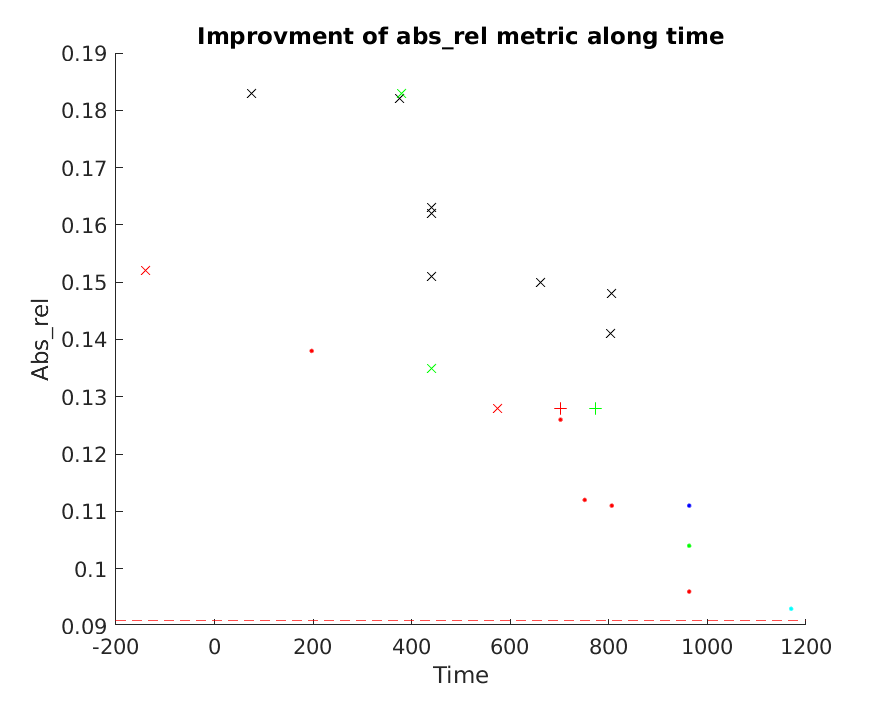
\includegraphics[width = \linewidth]{Rebuttal_MutualDepSegBenifits/Fig/abs_rel.png}
    \caption{Improvement of metric abs\_rel against submission time}
    \label{fig:abs_gain}
\end{figure}
\section*{Reviewer 2}
\subsection*{- - - - - - C2.1 \& C2.3 \& C2.4 \& C2.5 \& C2.6 - - - - - -}
\noindent\textbf{C2.1:} The experiments section discusses the benefits against [11] as baseline, when [38] should be used as baseline. This is easily amendable as authors have a comparable model trained for ablation study. \\
\noindent\textbf{C2.3:} The scores of (Baseline + $\mathbf{l_p}$) and (Baseline + M + $\mathbf{l_p}$) model in Table 4 are not as good as official scores of [38]. Is it because resolution difference, or different learning rate scheduling? Did you do "3 epoch fine-tuning" for the models in Table 4? \\
\noindent\textbf{C2.4:} Regarding the baselines in the experiments: The comparison in Tables 2 and 5, Figures 5, 6, 7 and 9 are against [11]. However, this is not a fair comparison, as [11] does not have $\mathbf{l_p}$ loss from [38]. The comparison should be against [38] as baseline in all of experiments. I think it is fine to use the method trained in Table 4 (Baseline + M + $\mathbf{l_p}$) for this (with an asterisk explaining these were trained by you) to measure the importance of $\mathbf{l_g}$. I think Figure 5 graph would make your model look quite comparable to Baseline + $\mathbf{l_p}$ model. \\ 
\noindent\textbf{C2.5:} The loss in Eq 13 is said to be applied to x where M(x)=0. Is this the case for all 3 terms of the loss? If so, then $\mathbf{l_g}$ is not being applied to occluded regions, where presumable it would be most useful? If not, then this equation needs to be updated. \\
\noindent\textbf{C2.6:} In Eq 16, you measure the reprojection error for morphed and predicted depth values. Under ideal semantic predictions the morphed depth would have higher reprojection error then predicted depth in the occluded regions, as explained in lines 407-420. So, the morphed depth would provide correct depth in the occluded regions, but the reprojection loss would be high in those regions as those regions are occluded in the stereo pair. Could you explain why this formulation of the loss does not causes issues with this line of reasoning and produces better boundaries around objects? \\ \\
\noindent\textbf{A:} We do not convey $\mathbf{l_p}$ special benefit in stabilizing training clearly, cause confusion. As unsupervised depth estimation requires additional constrain from different modality predictions, handling noise inside them will become increasing important. Comparing figure 8 column (d) and (e), we see $\mathbf{l_p}$ eliminate artifacts around foreground object. The artifact, as a joint result of noisy $\mathbf{l_g}$ and weak photometric supervision on those area(structural stereo occlusion and area is low-texture). In each iteration, as defined in line 477, no supervision signal imposed on Mask region. But the other side still receives supervision signal of $\mathbf{l_g}$. In addition, we do random flip during training, thus both side has 50\% probability get trained. However, noise inside segmentation and stereo occlusion mask $\mathbf{M}$, especially when prediction is bad at early stage, leading to artifacts. To avoid this, we include $\mathbf{l_p}$, which already uses good-quality stable prediction from SGM to help network robust to unstable early stage noise in prediction. This benefit was not rigorously discussed in previous work using SGM prediction, including [38]. We select [11] as baseline and treat $\mathbf{l_p}$ an additional loss to highlight this finding and inspire other researcher if facing similar difficulty. We mentioned this in supplementary material line 143-160 but not convey clearly, neither in fourth paragraph of ablation study nor method section line 511 - 518. We agree on doing comparison against baseline + $\mathbf{l_p}$ will be more fair in Tables 2, Figures 5, 6, 7, 9. We will update those figures, table and related paragraph in the final version. For Table 5, it is used to show generality of fine-tune strategy, better conducted against a public recognized method. In table 4, only the entry having "finetune" term includes the 3 epoch finetuning. We conclude performance difference against [38] to low quality SGM prediction. As at the time of our submission, the author of [38] does not public related parameter combination and iterate for optimal solution are time consuming.
\subsection*{- - - - - - - C2.2 - - - - - - -}
\noindent\textbf{C2.2:} The proposed approach is demonstrated for monocular depth estimation task trained from stereo. It could have been explored for related tasks such as optical flow or stereo matching. The paper does not discuss such opportunities and connections. \\ \\
\noindent\textbf{A:} In line 645 - 675, we also notice the sufficient space to explore and upgrade performance. But as we already use a quite complex training framework coupled with multiple losses, adding more, even though beneficial for performance, but make the paper less focus.
\subsection*{- - - - - - - C2.7 - - - - - - -}
\noindent\textbf{C2.7:} In Eq 16, How exactly do you measure Var(I)? What is the window for computing the variance? I'm assuming it is in a window, and not variance of color channels, as Var(I) represents the likelihood of the pixel belong to a textured region? \\ \\
\noindent\textbf{A:} Yes. It is the mean variance of RGB channels within a 3 x 3 window. It will be added to implementation details.
\subsection*{- - - - - - - C2.8 - - - - - - -}
\noindent\textbf{C2.8:} The improvements in Table 3 are very small for supervised and stereo methods, only RMSE seems to have more significant improvements. Why is that? Are these models already sharp around boundaries and semantic segmentation is not useful? \\ \\
\noindent\textbf{A:} We are optimizing the border in a "greedy search" manner. The results listed in Table 3 can be viewed as benefits gained after a single greedy search, which is expected to be small. And after each morphing, the depth gradient along the border will be reduced to $\frac{t}{1 + t}$(can be viewed in supp equation 3), thus we can not adjust the border of depth to semantic only relying on the morph. In this regard, the benefits brought by morph can not be used to reflect border quality contrast between depth and semantics, unable to indicate they are "good enough".
\section*{Reviewer 1}
\subsection*{- - - - - - - C1.1 - - - - - - -}
\noindent\textbf{C1.1:} In Eq9, why is h() not part of weight normalization? Why this choice ? \\ \\
\noindent\textbf{A:} $h()$ controls range of single semantic-edge pair, independent of the number. $w()$ controls mutual relationships across multiple pairs. Consider when only one pair exists, if both normalized, then every pixel within the image will be affected by the pair, which is unreasonable. 
\subsection*{- - - - - - - C1.2 - - - - - - -}
\noindent\textbf{C1.2:} Sec 3.2 gives an explanation for bleeding which only covers bleeding to the left side of an object. But the bleeding artifact is present in all directions. What helps the up/down bleeding in the proposed algorithm? \\ \\
\noindent\textbf{A:} Up-down bleeding artifacts can be viewed as a series of left-right bleeding artifacts, whose largest center disparity value decreasing in vertical direction. Then up-down artifacts are automatically handled by mask dealing with left-right artifacts. For example, in figure 4.c, occlusion mask already cover the top blobbed border of the object. But we do not think, for example, the fading head in supplementary figure 4 row 2, column 1 as bleeding artifacts. It is a common flaw of neural network failing to recover high frequency details, which is dealt via proposed $l_p$ loss. The figure 4 row2, column 2, after adding $l_p$, it is relieved.
\subsection*{- - - - - - - C1.3 - - - - - - -}
\noindent\textbf{C1.2:} Comparison in Table 2 would be fair if the authors use Resnet18 since [11] uses it. I would recommend adding this row to benefit the paper. Similarly, for fig5. \\ \\
\noindent\textbf{A:} Yes we agree, that is more fair.
{\small
\bibliographystyle{ieee}
\bibliography{egbib}
}

\end{document}
